\documentclass[10pt, a4paper]{article}
\usepackage[slovene]{babel}
\usepackage[T1]{fontenc}
\usepackage[utf8]{inputenc}
\usepackage{lmodern}
\usepackage{amsmath}
\usepackage{amsthm}
\usepackage{amssymb}
\usepackage{pgfplots}
\usepackage{comment}
\usepackage{graphicx}
\usepackage{booktabs}
\usepackage{array} 
\usepackage{comment}
\usepackage{tikz}
\usepackage{pythonhighlight}
\usepackage{listings} %code extracts
\usepackage{xcolor} %custom colours
\usepackage{mdframed} %nice frames
\usepackage{float}
\usepackage{siunitx}

\definecolor{light-gray}{gray}{0.95} %the shade of grey that stack exchange uses

%Put in the main document
\newenvironment{coutput}{\begin{mdframed}[backgroundcolor=light-gray, roundcorner=10pt,leftmargin=1, rightmargin=1, innerleftmargin=15, innertopmargin=15,innerbottommargin=15, outerlinewidth=1, linecolor=light-gray]
\begin{lstlisting}}{\end{lstlisting}
\end{mdframed} }

\tikzset{every picture/.style={line width=0.75pt}} %set default line width to 0.75pt    

{\theoremstyle{plain}
\newtheorem{izrek}{Izrek}[section]
\newtheorem{zgled}[izrek]{Zgled}
\newtheorem{trditev}[izrek]{Trditev}
\newtheorem{posledica}[izrek]{Posledica}
\newtheorem{lema}[izrek]{Lema}
}

{\theoremstyle{definition}
\newtheorem{definicija}[izrek]{Definicija}
}

{\theoremstyle{remark}
\newtheorem*{opomba}{Opomba}
\newtheorem*{dogovor}{Dogovor}
}

\newcommand{\N}{\mathbb {N}}
\newcommand{\Z}{\mathbb {Z}}
\newcommand{\Q}{\mathbb {Q}}
\newcommand{\R}{\mathbb {R}}
\newcommand{\C}{\mathbb {C}}
\newcommand{\F}{\mathbb {F}}
\newcommand{\Ha}{\mathbb {H}}
\newcommand{\prob}{\mathbb {P}}
\newcommand{\E}{\mathbb {E}}
\newcommand{\zap}[1]{(#1_n)_{n=1} ^{\infty}}
\newcommand{\podzap}[1]{(#1_{n_j})_{n=1 ^{\infty}}}
\newcommand{\limzap}[1]{\lim_{n \to \infty} {#1}}
\newcommand{\limf}[3]{\lim_{#1 \to #2} {#3}}
\newcommand{\rlimf}[3]{\lim_{#1 \downarrow #2} {#3}}
\newcommand{\llimf}[3]{\lim_{#1 \uparrow #2} {#3}}
\newcommand{\quot}[2]{{\raisebox{0em}{$#1$}\left/\raisebox{0em}{$#2$}\right.}}
\newcommand{\gen}[1]{\left\langle #1 \right\rangle}
\newcommand{\Mod}[1]{\ (\mathrm{mod}\ #1)}
\DeclareMathOperator{\cov}{cov}
\DeclareMathOperator{\var}{var}
\DeclareMathOperator{\se}{SE}
\DeclareMathOperator{\sd}{SD}

\begin{document}

\title{Projektna naloga iz statistike}
\author{Gal Anton Gorše}
\maketitle

Projektna naloga je bila rešena v programskem jeziku Python s pomočjo knjižnice Pandas.

\tableofcontents

\clearpage

\section*{Prva naloga}
\addcontentsline{toc}{section}{\protect\numberline{}Prva naloga}

Zanima nas število otrok v družinah. Imamo populacijo $m$ družin, katerih povprečje je 
$$\mu = \frac{x_1 + x_2 + \dots + x_m}{m},$$
varianca pa 
$$\sigma^2 = \frac{(x_1 - \mu)^2 + (x_2 - \mu)^2 + \dots + (x_m - \mu)^2}{m},$$
kjer smo z $x_i$ označili število otrok $i$-te družine.

\begin{python}
    kibergrad = pd.read_csv("Kibergrad.csv")
    m = len(kibergrad.index)
    otroci = kibergrad["'OTROK'"]
    globalno_povprecje = otroci.mean()
    print(globalno_povprecje)
\end{python}

\begin{python}
    0.9479332816843641
\end{python}


\subsection*{(a)}
\addcontentsline{toc}{subsection}{\protect\numberline{}(a)}

Vzamemo vzorec $200$ družin
$$(X_1, X_2, \dots, X_{200}).$$
Vemo, da je povprečje njihovih števil otrok nepristranska cenilka za $\mu$:
$$\overline{X} = \frac{X_1 + X_2 + \dots + X_{200}}{200}.$$
Če to izračunamo:
\begin{python}
    kibergrad = pd.read_csv("Kibergrad.csv")
    otroci = kibergrad["'OTROK'"]
    m = len(kibergrad.index)
\end{python}
dobimo rezultat
\begin{python}
    0.975
\end{python}

\subsection*{(b)}
\addcontentsline{toc}{subsection}{\protect\numberline{}(b)}

Vemo, da je kvadrat standardne napake $\hat{\mu}$ pri enostavnem slučajnem vzorčenju 
z $n$ elementi enak 
$$\se_{\overline{X}} ^2 = \frac{m - n}{m - 1} \frac{\sigma^2}{n}.$$
Če uporabimo nepristransko cenilko za varianco
$$\widehat{\sigma^2} = \frac{m - 1}{m} \frac{1}{n - 1} \sum_{i = 1}^n (X_i - \overline{X})^2,$$
dobimo nepristransko cenilko 
$$\widehat{\se ^2}_{\overline{X}} = \frac{m - n}{m} \frac{1}{n(n - 1)} \sum_{i = 1}^n (X_i - \overline{X})^2.$$
Tako dobimo tudi cenilko 
$$\widehat{\se}_{\overline{X}} = \sqrt{\frac{m - n}{mn}}  \sqrt{\frac{1}{(n - 1)} \sum_{i = 1}^n (X_i - \overline{X})^2},$$
ki sicer ni več nepristranska, je pa še zmerom dovolj dobra.
Iz knjige \cite{rice} sledi, da če je $n$ velik, ampak še zmerom majhen glede na $m$,
potem je $\overline{X}$ porazdeljen približno normalno. Od tod dobimo aproksimativni interval zaupanja:
$$\overline{X} - \se_{\overline{X}} \cdot \Phi^{-1} \left(1 - \frac{\alpha}{2}\right) \leq \mu \leq \overline{X} + \se_{\overline{X}} \cdot \Phi^{-1} \left(1 - \frac{\alpha}{2}\right).$$
Ponavadi ne poznamo dejanske $\se_{\overline{X}}$, zato uporabimo cenilko $\widehat{\se}_{\overline{X}}$. Tako dobimo interval zaupanja
$$\overline{X} - \widehat{\se}_{\overline{X}} \cdot \Phi^{-1} \left(1 - \frac{\alpha}{2}\right) \leq \mu \leq \overline{X} + \widehat{\se}_{\overline{X}} \cdot \Phi^{-1} \left(1 - \frac{\alpha}{2}\right).$$

\begin{python}
    cenilka_se = math.sqrt((m - 200)/(200*m))*vzorec.std()
    c = norm.ppf(0.975)
    delta = c*cenilka_se
    print(povprecje - delta, povprecje + delta)
\end{python}

\begin{python}
    0.8179002058696819 1.132099794130318
\end{python}

Tako dobimo $95\%$ interval zaupanja:
$$0.82 \leq \mu \leq 1.13.$$

\subsection*{(c) in (d)}
\addcontentsline{toc}{subsection}{\protect\numberline{}(c) in (d)}

Zgornji potek konstrukcije $95\%$ intervala zaupanja ponovimo na $100$ vzorcih.

\begin{python}
    x = np.arange(100)
    pomozni_x = np.linspace(0, 100, 1000)
    podatki = np.empty(100)
    intervali = np.empty(100)
    stevec = 0

    for i in range(100):
        zacasni_vzorec = otroci.sample(200)
        zacasno_povprecje = zacasni_vzorec.mean()
        zacasna_se = math.sqrt((m - 200)/(200*m))*zacasni_vzorec.std()
        podatki[i] = zacasno_povprecje
        intervali[i] = zacasna_se
        if abs(zacasno_povprecje - globalno_povprecje) <= zacasna_se*c:
            stevec += 1

    fig, ax = plt.subplots()
    plt.errorbar(x, podatki, yerr=intervali*c, fmt="none")
    plt.plot(pomozni_x, globalno_povprecje*np.ones(1000), "r")
    ax.grid(False)
    ax.set_xlabel("Intervali")
    plt.tight_layout()
    plt.show()
    print(stevec)
\end{python}

\begin{python}
    96
\end{python}

\begin{figure}[H]
    \centering
    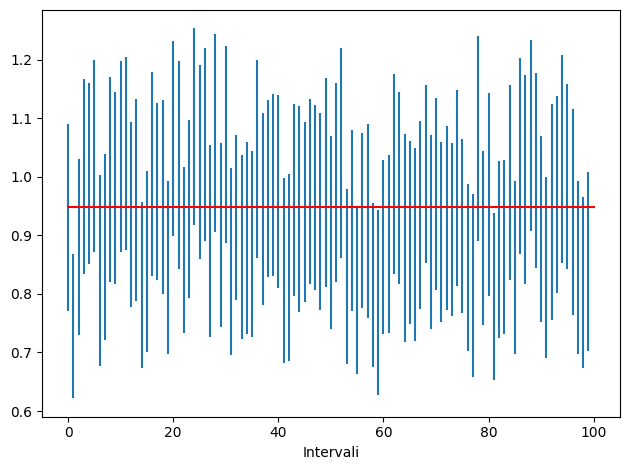
\includegraphics[scale=0.75]{Images/1c.png}
    \caption{Intervali zaupanja za $\mu$ za vzorce velikosti $n = 200$}
\end{figure}

Vidimo, da je povprečje populacije $\mu$ vsebovano v $96$ intervalih zaupanja.

\subsection*{(e)}
\addcontentsline{toc}{subsection}{\protect\numberline{}(e)}

Standardna napaka cenilke $\overline{X}$ za vzorce velikosti $200$ je 
$$\se_{\overline{X}} = \sqrt{\frac{m - 200}{m - 1}} \frac{\sigma}{\sqrt{200}}$$
(glej točko (b)). Po definiciji je $\se_{\overline{X}} = \sqrt{\var(\overline{X})} = \sigma_{\overline{X}}$,
kar pa je natanko standardna deviacija slučajne spremenljivke $\overline{X}$.
Označimo povprečje $i$-tega vzorca iz točke (d) z $\overline{X}_i$.
Očitno so $\overline{X}_1, \overline{X}_2, \dots, \overline{X}_k$ neodvisne enako porazdeljene slučajne spremenljivke.
Empirična standardna deviacija vzorčnih povprečij je enaka
$$\widehat{\sigma}_{\overline{X}} = \sqrt{\frac{1}{k} \sum_{i = 1} ^{k} \left(\overline{X}_i - \frac{1}{k}\sum_{j = 1} ^k \overline{X}_j\right)^2}.$$
Iz predavanj vemo, da je $\widehat{\sigma}_{\overline{X}}$ dosledna cenilka za standardno deviacijo 
$\sigma_{\overline{X}}$, torej gre $$\widehat{\sigma}_{\overline{X}} \xrightarrow[k \to \infty]{d} {\sigma_{\overline{X}}} = \se_{\overline{X}}.$$
Pričakujemo lahko torej, da bosta za $k = 100$ izračunani vrednosti $\se_{\overline{X}}$ ter $\widehat{\sigma}_{\overline{X}}$ dovolj blizu.
Pa jih izračunajmo.

\begin{python}
    dejanska_se = math.sqrt((m - 200)/(200*(m - 1)))*otroci.std(ddof=0)
    sd_povprecij = math.sqrt(sum((podatki - podatki.mean()*np.ones(100))*(podatki - podatki.mean()*np.ones(100)))*(1/100))
    print(dejanska_se, sd_povprecij)
\end{python}

\begin{python}
    0.0816404987959038 0.07567725880342124
\end{python}

Tako dobimo $\se_{\overline{X}} = 0.082$ in $\widehat{\sigma}_{\overline{X}} = 0.076$.

\subsection*{(f)}
\addcontentsline{toc}{subsection}{\protect\numberline{}(f)}

Ponovimo prejšnji dve točki še za vzorce velikosti $n = 800$.

\begin{python}
    podatki_alt = np.empty(100)
    intervali_alt = np.empty(100)
    stevec_alt = 0

    for i in range(100):
        zacasni_vzorec = otroci.sample(800)
        zacasno_povprecje = zacasni_vzorec.mean()
        zacasna_se = math.sqrt((m - 800)/(800*m))*zacasni_vzorec.std()
        podatki_alt[i] = zacasno_povprecje
        intervali_alt[i] = zacasna_se
        if abs(zacasno_povprecje - globalno_povprecje) <= zacasna_se*c:
            stevec_alt += 1

    fig, ax = plt.subplots()
    plt.errorbar(x, podatki_alt, yerr=intervali_alt*c, fmt="none")
    plt.plot(pomozni_x, globalno_povprecje*np.ones(1000), "r")
    ax.grid(False)
    ax.set_xlabel("Intervali")
    plt.tight_layout()
    plt.show()
    print(stevec_alt)
\end{python}

\begin{python}
    96
\end{python}

\begin{figure}[H]
    \centering
    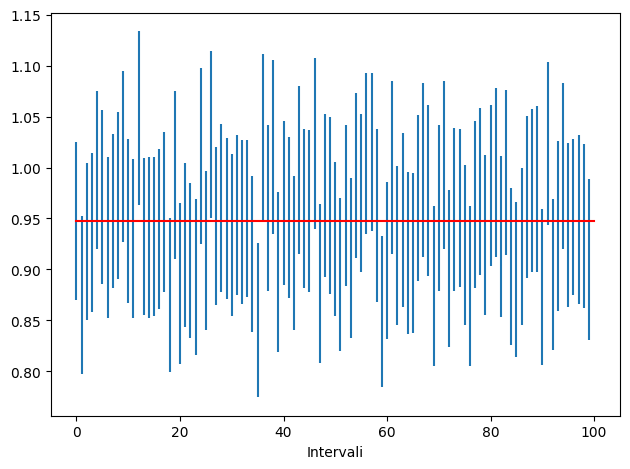
\includegraphics[scale=0.75]{Images/1f.png}
    \caption{Intervali zaupanja za $\mu$ za vzorce velikosti $n = 800$}
\end{figure}

Izračunajmo še $\se_{\overline{X}}$ ter $\sigma_{\overline{X}}$.

\begin{python}
    dejanska_se_alt = math.sqrt((m - 800)/(800*(m - 1)))*otroci.std(ddof=0)
    sd_povprecij_alt = math.sqrt(sum((podatki_alt - podatki_alt.mean()*np.ones(100))*(podatki_alt - podatki_alt.mean()*np.ones(100)))*(1/99))
    print(dejanska_se_alt, sd_povprecij_alt)
\end{python}

\begin{python}
    0.040538959874385 0.042084231538569404
\end{python}

Dobimo torej, da je $\se_{\overline{X}} = 0.041$ in $\sigma_{\overline{X}} = 0.042$.
Takoj opazimo, da je standardna napaka pri $n = 800$ manjša kot pri $n = 200$ in so intervali zaupanja
na grafu krajši. To smo pričakovali,
saj je jasno, da z večjimi vzorci dobimo boljšo napoved. 
Sledi pa tudi iz formule za standardno napako: če sta $n_1 < n_2$ naravni števili, potem je 
\begin{align*}
    \se_{\overline{X}} ^{(n = n_1)} &= \sqrt{\frac{m - n_1}{m - 1}} \frac{\sigma}{\sqrt{n_1}}\\
    &\geq \sqrt{\frac{m - n_2}{m - 1}} \frac{\sigma}{\sqrt{n_2}}\\
    &= \se_{\overline{X}} ^{(n = n_2)}.
\end{align*}
Opazimo tudi, da je standardna napaka $\se_{\overline{X}} ^{(n = 200)}$ približno dvakrat večja od $\se_{\overline{X}} ^{(n = 800)}$.
To lahko utemeljimo tudi računsko.
\begin{align*}
    \frac{\se_{\overline{X}} ^{(n = 200)}}{\se_{\overline{X}} ^{(n = 800)}} &= \frac{\sqrt{\frac{m - 200}{m - 1}} \frac{\sigma}{\sqrt{200}}}{\sqrt{\frac{m - 800}{m - 1}} \frac{\sigma}{\sqrt{800}}}\\
    &= \sqrt{\frac{m - 200}{m - 800}} \sqrt{\frac{800}{200}}\\
    &\approx 2.
\end{align*}
V splošnem velja, da če je $m >> n$, potem pri množenju $n$ s faktorjem $k$ standardna napaka 
vzorčnega povprečja zmanjša za približno faktor $\sqrt{k}$.

\section*{Druga naloga}
\addcontentsline{toc}{section}{\protect\numberline{}Druga naloga}

Podanih imamo $n$ meritev $x_1, x_2, \dots, x_n$.
Označimo vrstilno statistiko 
$$x_{(1)} \leq x_{(2)} \leq \dots \leq x_{(n)}.$$

\begin{python}
    mangan = pd.read_csv("Mangan.csv")
    mangan = pd.DataFrame(
        mangan[["'ODLITEK1\'", "'ODLITEK2\'", 
        "'ODLITEK3\'", "'ODLITEK4\'", "'ODLITEK5\'"]]
            .unstack().reset_index(drop=True), 
            columns=["ODLITEK"])

    odlitek = mangan["ODLITEK"]
    n = len(odlitek)
\end{python}

\subsection*{(a)}
\addcontentsline{toc}{subsection}{\protect\numberline{}(a)}

Najprej izračunamo interkvartilni razmik 
$$\mathrm{IQR} = x^+ _{\frac{3}{4}} - x^- _{\frac{1}{4}} = 0.18$$
s pomočjo katerega dobimo širino za modificirano Freedman-Diaconisovo pravilo:
$$\mathrm{širina} = \frac{2.6 \cdot \mathrm{IQR}}{\sqrt[3]{n}} = 0.09.$$
Od tod dobimo število stolpcev v histogramu:
$$\left\lfloor \frac{x_{(n)} - x_{(1)}}{\mathrm{širina}} \right\rfloor + 1 = 9.$$
Nadalje izračunamo povprečje meritev
$$\widehat{\mu} = \frac{x_1 + x_2 + \dots + x_n}{n} = 1.41$$
in popravljeni vzorčni standardni odklon 
$$\widehat{\sigma}_+ = \sqrt{\frac{1}{n - 1} \sum_{i = 1} ^n (x_i - \widehat{\mu})^2} = 0.15.$$
Ti statistiki bomo potrbovali za primerjavo empirične porazdelitve s teoretično (normalno) porazdelitvijo.

\begin{figure}[H]
    \centering
    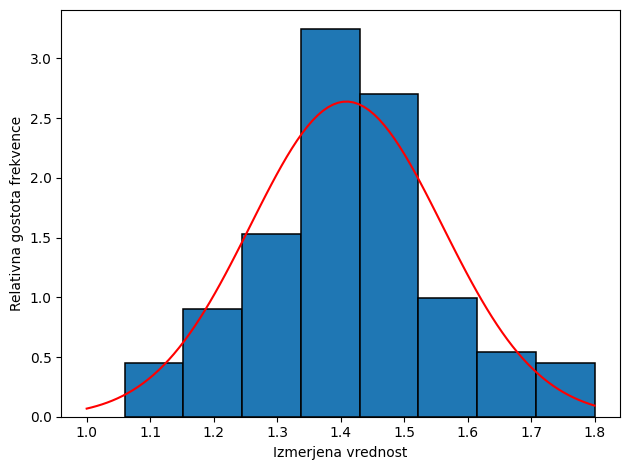
\includegraphics[scale=0.75]{Images/2a.png}
    \caption{Histogram po modificiranem Freedman-Diaconisovem pravilu}
\end{figure}

Poglejmo si kodo.

\begin{python}
    Q1, Q3 = odlitek.quantile([.25, .75])
    IQR = Q3 - Q1
    sirina = 2.6 * IQR / pow(120, 1/3)
    stevilo = int((odlitek.max() - odlitek.min())/sirina + 1)
    mi, sigma = odlitek.mean(), odlitek.std()

    fig, ax = plt.subplots(nrows=1, ncols=1)
    ax.hist(odlitek, stevilo, density=True, edgecolor="black", linewidth=1.1)
    ax.set_xlabel("Izmerjena vrednost")
    ax.set_ylabel("Relativna gostota frekvence")
    ax.grid(False)
    x = np.linspace(1.0, 1.8, 100)
    plt.plot(x, stats.norm.pdf(x, mi, sigma), "r")
    plt.tight_layout()
    plt.show()
    print(IQR, sirina, mi, sigma)
\end{python}

\begin{python}
    0.17999999999999994 0.09488235113094502 1.409 0.151182454186263
\end{python}

\subsection*{(b)}
\addcontentsline{toc}{subsection}{\protect\numberline{}(b)}

Empirično porazdelitev želimo podrobneje primerjati z normalno.
Denimo, da razdelimo vrednosti na $k$ intervalov, pri čemer ima $i$-ti 
levo krajišče $y_{i - 1}$ in desno $y_i$. Označimo z $n_i$ frekvenco 
ponovitev v $i$-tem intervalu ter definiramo relativno frekvenco $p_i = \frac{n_i}{n}$.
Ker empirično porazdelitev primerjamo z normalno, definiramo še teoretično relativno frekvenco 
$$\widehat{p_i} = \Phi \left(\frac{y_i - \widehat{\mu}}{\widehat{\sigma}_+}\right) - \Phi \left(\frac{y_{i - 1} - \widehat{\mu}}{\widehat{\sigma}_+}\right)$$
in teoretično frekvenco $\widehat{n_i} = n \widehat{p_i}$. 
Ker je $n_i$ empirična slučajna spremenljivka, velja 
\begin{align*}
    \var (n_i - \widehat{n_i}) &= \var(n_i)\\
    &= n p_i (1 - p_i)\\
    &= np_i - np_i^2\\
    &\approx np_i,
\end{align*}
pri čemer smo predpostavili, da so relativne gostote dovolj majhne.
To nam pove, da je variabilnost $n_i - \widehat{n_i}$ večja v tistih intervalih,
kjer je $p_i$ večja. Denimo, da bi narisali histogram, kjer ima $i$-ti interval 
stolpec z višino $n_i - \widehat{n_i}$. 
Ker je variabilnost razlikuje od intervala do intervala, je težko oceniti, 
kdaj gre za dejansko odstopanje od modela.

Rešitev je naslednja. Denimo, da ima naključna spremenljivka $X$ povprečje $\mu$
in varianco $\sigma^2 (\mu)$, ki je odvisna le od $\mu$. Če je $Y = f(X)$, potem iz \cite{rice} sledi 
$$\var (Y) \approx \sigma^2 (\mu) (f'(\mu))^2.$$
V našem primeru je 
$$\mu = \E(n_i) = np_i \approx \var (n_i) = \sigma^2 (\mu).$$
Najti želimo tako funkcijo $f$, da je $\mu (f'(\mu))^2$ konstanta.
Taka funkcija je recimo $f(x) = \sqrt{x}$. Zato narišemo histogram, katerega stolpci so višine 
$\sqrt{n_i} - \sqrt{\widehat{n_i}}$.

Najprej naredimo primer, ko za vsako vrednost narišemo samostojen stolpec.

\begin{python}
    x = np.linspace(1.05, 1.81, 39)
    x_mid = (x[1:] + x[:-1])/2
    frekvence = mangan.value_counts()
    koreni_razlik = np.empty(38)
    stevec = 0
    for i in x_mid:
        pricakovana_frekvenca = (stats.norm.cdf((i+ 0.01 - mi)/sigma) - stats.norm.cdf((i- 0.01 - mi)/sigma))*n
        if stevec == 0:
            dejanska_frekvenca = len(odlitek[odlitek.between(x[stevec], x[stevec + 1])])
        else:
            dejanska_frekvenca = len(odlitek[odlitek.between(x[stevec], x[stevec + 1], inclusive="right")])
        koreni_razlik[stevec] = math.sqrt(dejanska_frekvenca) - math.sqrt(pricakovana_frekvenca)
        stevec += 1

    fig, ax = plt.subplots(nrows=1, ncols=1)
    ax.bar(x_mid, koreni_razlik, width=0.02, bottom=None, align='center', edgecolor="black", linewidth=1.1)
    ax.grid(False)
    ax.set_xlabel("Izmerjena vrednost")
    ax.set_ylabel("Razlika korenov frekvenc")
    plt.tight_layout()
    plt.show()
\end{python}

\begin{figure}[H]
    \centering
    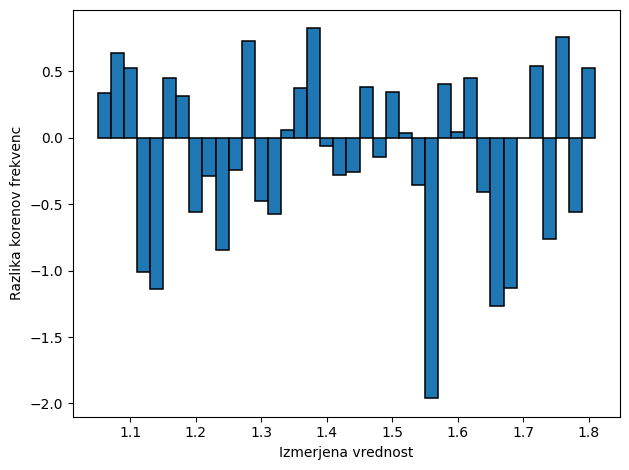
\includegraphics[scale=0.75]{Images/2bi.png}
    \caption{Viseči histogram razlik korenov frekvenc}
\end{figure}

Sedaj si pa še poglejmo primer, ko izberemo širino intervalov po modificiranem
Freedman-Diaconisovem pravilu kot v prejšnji točki.

\begin{python}
    x_alt = np.linspace(1.06, 1.80, 9)
    x_alt_mid = (x_alt[1:] + x_alt[:-1]) / 2
    koreni_razlik_alt = np.empty(8)
    stevec_alt = 0
    for i in x_alt_mid:
        pricakovana_frekvenca = (stats.norm.cdf((i + (0.74/8)/2 - mi)/sigma) - stats.norm.cdf((i - (0.74/8)/2 - mi)/sigma))*n
        if stevec_alt == 0:
            dejanska_frekvenca = len(odlitek[odlitek.between(x_alt[stevec_alt], x_alt[stevec_alt + 1])])
        else:
            dejanska_frekvenca = len(odlitek[odlitek.between(x_alt[stevec_alt], x_alt[stevec_alt + 1], inclusive="right")])
        koreni_razlik_alt[stevec_alt] = math.sqrt(dejanska_frekvenca) - math.sqrt(pricakovana_frekvenca)
        stevec_alt += 1

    fig, ax = plt.subplots(nrows=1, ncols=1)
    ax.bar(x_alt_mid, koreni_razlik_alt, 0.74/8, bottom=None, align='center', edgecolor="black", linewidth=1.1)
    ax.set_xlabel("Izmerjena vrednost")
    ax.set_ylabel("Razlika kvadratov frekvenc")
    ax.grid(False)
    plt.tight_layout()
    plt.show()
\end{python}

\begin{figure}[H]
    \centering
    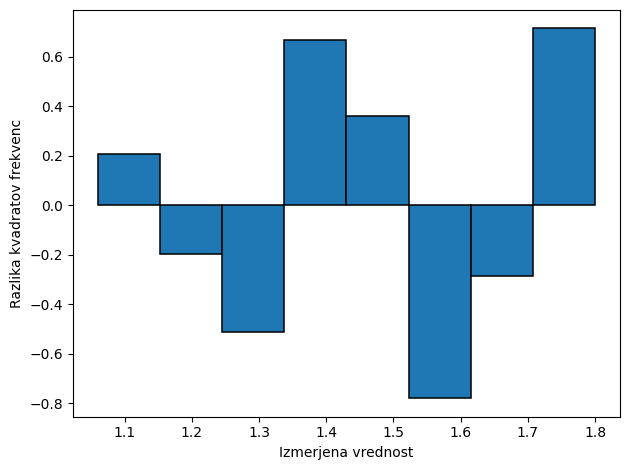
\includegraphics[scale=0.75]{Images/2bii.png}
    \caption{Viseči histogram razlik kvadratov frekvenc pri MFD}
\end{figure}

\subsection*{(c)}
\addcontentsline{toc}{subsection}{\protect\numberline{}(c)}

V Q-Q grafikonu prikažemo urejena opažanja proti kvantilom teoretične (v našem primeru seveda normalne)
porazdelitve za $\frac{1}{n + 1}, \dots, \frac{n}{n + 1}$.

\begin{python}
    fig, ax = plt.subplots(nrows=1, ncols=1)
    stats.probplot(odlitek, dist="norm", plot=plt)
    ax.set_title(None)
    ax.set_xlabel("Kvantil normalne porazdelitve")
    ax.set_ylabel("Meritev")
    ax.grid(False)
    plt.tight_layout()
    plt.show()
\end{python}

\begin{figure}[H]
    \centering
    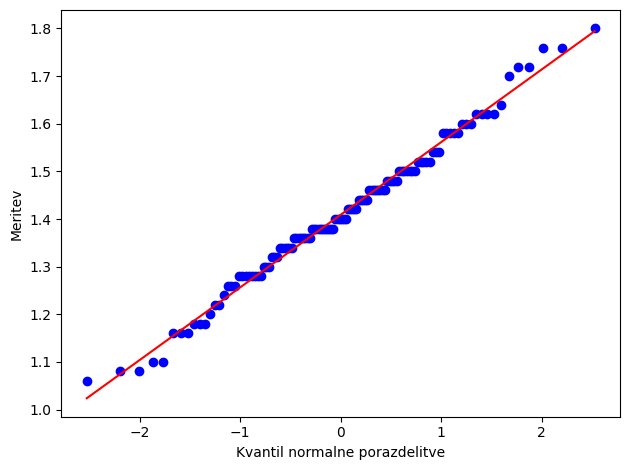
\includegraphics[scale=0.75]{Images/2c.png}
    \caption{Q-Q grafikon za normalno porazdelitev}
\end{figure}

\section*{Tretja naloga}
\addcontentsline{toc}{section}{\protect\numberline{}Tretja naloga}

V tej nalogi imamo podanih $n$ meritev dolžin odontoblastov morskih prašičkov in količino C 
vitamina, ki so jo prejeli (v obliki VC ali OJ).

\begin{python}
    zobje = pd.read_csv("Zobje.csv")
    zobje_vc = (zobje[zobje["NACIN"]=="VC"])[["DOLZINA", "KOLICINA"]]
    zobje_oj = (zobje[zobje["NACIN"]=="OJ"])[["DOLZINA", "KOLICINA"]].reset_index(drop=True)

    def nacin(x):
        if x == "VC":
            return 0.0
        else:
            return 1.0

    zobje["NACIN"] = zobje["NACIN"].apply(lambda x: nacin(x))
    zobje["NACIN*KOLICINA"] = zobje["NACIN"]*zobje["KOLICINA"]
    n = length(zobje)
\end{python}

\subsection*{(a)}
\addcontentsline{toc}{subsection}{\protect\numberline{}(a)}

V prvem delu naloge privzamemo linearni model 
$$\mathrm{dolžina} = \beta_0 + \beta_1 \cdot \mathrm{količina} + \varepsilon.$$
Denimo, da je $x_i$ količina odmerka vitamina C (bodisi v obliki VC bodisi OJ)
na $i$-temu morskemu prašičku in $Y_i$ njegova izmerjena dolžina odontoblastov.
Imamo torej 
$$\underbrace{\begin{bmatrix}
    Y_1\\
    Y_2\\
    \vdots\\
    Y_{60}
\end{bmatrix}}_{\underline{Y}} = \underbrace{\begin{bmatrix}
    1 & x_1\\
    1 & x_2\\
    \vdots & \vdots\\
    1 & x_{60}
\end{bmatrix}}_{\underline{X}} \cdot \underbrace{\begin{bmatrix}
    \beta_0\\
    \beta_1
\end{bmatrix}}_{\underline{\beta}} + \underbrace{\begin{bmatrix}
    \varepsilon_1\\
    \varepsilon_2\\
    \vdots\\
    \varepsilon_{60}
\end{bmatrix}}_{\underline{\varepsilon}},$$
kjer za šum velja $\E (\underline{\varepsilon}) = 0$ in $\underline{\varepsilon} \sim N(0, \sigma^2 \underline{I}_{60})$.

Iz predavanj vemo, da je cenilka za $\underline{\beta}$ 
$$\widehat{\underline{\beta}} = (\underline{X}^\top \underline{X})^{-1} \underline{X}^\top \underline{Y}.$$
Označimo 
$$\mathrm{RSS} = \|\underline{Y}  - \underline{X} \underline{\widehat{\beta}}\|^2.$$
Na predavanjih smo pokazali, da je 
$$\widehat{\sigma_+^2} = \frac{\mathrm{RSS}}{n - 2}$$
nepristranska cenilka za $\sigma^2$ in za poljuben vektor $\underline{c} \in \R^2$
velja 
$$\frac{\underline{c}^\top \widehat{\underline{\beta}} - \underline{c}^\top \underline{\beta}}{\widehat{\se}_+} \sim \mathrm{Student} (n - 2),$$
kjer je 
\begin{equation}
    \widehat{\se}_+ = \widehat{\sigma}_+ \sqrt{\underline{c}^\top (\underline{X}^\top \underline{X})^{-1} \underline{c}}. \label{eq:1}
\end{equation}

Testiramo, če je $\beta_1 = 0$; naša ničelna hipoteza je torej 
$$H_0:\ \beta_1 = 0,$$
ki jo moramo zavrniti z $100(1 - \alpha)\%$ verjetnostjo.
Alternativna hipoteza je zato seveda $$H_1:\ \beta_1 \neq 0.$$
V enačbi \eqref{eq:1} torej vzamemo $$\underline{c} = \begin{bmatrix}
    0\\ 1
\end{bmatrix}$$ in dobimo 
$$\frac{\widehat{\beta_1} - \beta_1}{\widehat{\se}_+} \sim \mathrm{Student} (n - 2).$$
Ničelne hipoteze torej ne zavrnemo natanko tedaj, ko je 
$$-F^{-1}_{\mathrm{Student} (n - 2)} \left(1 - \frac{\alpha}{2}\right) \leq \frac{\widehat{\beta_1}}{\widehat{\se}_+} \leq F^{-1}_{\mathrm{Student} (n - 2)} \left(1 - \frac{\alpha}{2}\right)$$
oziroma 
$$\left| \frac{\widehat{\beta_1}}{\widehat{\se}_+} \right| \leq F^{-1}_{\mathrm{Student} (n - 2)} \left(1 - \frac{\alpha}{2}\right).$$
Ker je funkcija gostote $F_{\mathrm{Student} (n - 2)}$ naraščajoča, lahko to zapišemo tudi kot 
$$F_{\mathrm{Student} (n - 2)} \left(\left| \frac{\widehat{\beta_1}}{\widehat{\se}_+} \right|\right) \leq 1 - \frac{\alpha}{2}.$$
Zaradi simetričnosti velja $F_{\mathrm{Student} (n - 2)} (x) = 1 - F_{\mathrm{Student} (n - 2)}(-x)$, zato je zgornja neenakost ekvivalentna 
$$F_{\mathrm{Student} (n - 2)} \left(\left| \frac{\widehat{\beta_1}}{\widehat{\se}_+} \right|\right) - F_{\mathrm{Student} (n - 2)} \left(-\left| \frac{\widehat{\beta_1}}{\widehat{\se}_+} \right|\right) \leq 1 - \alpha.$$
To pa pomeni, da je 
$$\prob \left(-\left| \frac{\widehat{\beta_1}}{\widehat{\se}_+} \right| \leq X \leq \left| \frac{\widehat{\beta_1}}{\widehat{\se}_+} \right|\right) \leq 1 - \alpha,\quad X \sim \mathrm{Student} (n - 2)$$
oziroma
$$\alpha \leq 1 - \prob \left(-\left| \frac{\widehat{\beta_1}}{\widehat{\se}_+} \right| \leq X \leq \left| \frac{\widehat{\beta_1}}{\widehat{\se}_+} \right|\right),\quad X \sim \mathrm{Student} (n - 2).$$
Izrazu na desni strani neenakosti pravimo $p$-vrednost. Ničelne hipoteze ne zavrnemo,
če je $\alpha \leq p$, sicer pa jo. Sedaj izvedemo test.

\begin{python}
    neodvisna = zobje["KOLICINA"]
    odvisna = zobje["DOLZINA"]
    neodvisna = sm.add_constant(neodvisna)
    reg = sm.OLS(odvisna, neodvisna).fit()
    koef = reg.params
    print(reg.summary())
    c0, c1 = koef["const"], koef["KOLICINA"]

    x = np.linspace(0.5, 2.0, 100)
    fig, ax = plt.subplots()
    ax.set_facecolor('white')
    plt.scatter(zobje["KOLICINA"], zobje["DOLZINA"], c="purple")
    plt.plot(x, c0 * np.ones(100) + c1 * x, "purple")
    ax.set_xlabel("Kolicina vitamina C")
    ax.set_ylabel("Dolzina odontoblastov")
    ax.grid(False)
    plt.tight_layout()
    plt.show()
\end{python}

Dobimo rezultat:

\begin{figure}[H]
    \centering
    \begin{tabular}{lSSSSSS} \toprule
        & $\mathrm{coef}$ & $\mathrm{std\ err}$ & {$t$} & {$P > |t|$} & {$0.025$} & {$0.975$} \\ \midrule
        const  & 7.4225 & 1.260 & 5.890 & 0.000 & 4.900 & 9.945 \\
        KOLICINA  & 9.7636  & 0.953 & 10.250 & 0.000 & 7.857 & 11.670 \\ 
        \bottomrule
    \end{tabular}   
    \caption{Tabela koeficientov v regresijskem modelu iz točke (a)} 
\end{figure}

Ker je $p$-vrednost v stolpcu KOLICINA zelo majhna, zavrnemo ničelno hipotezo tako v primeru 
$\alpha = 0.05$ kot tudi v primeru $\alpha = 0.01$ in sprejmemo alternativno hipotezo $H_1$.
Prišli smo do zaključka, da dodajanje vitamina C vpliva na dolžino odontoblastov.

\begin{figure}[H]
    \centering
    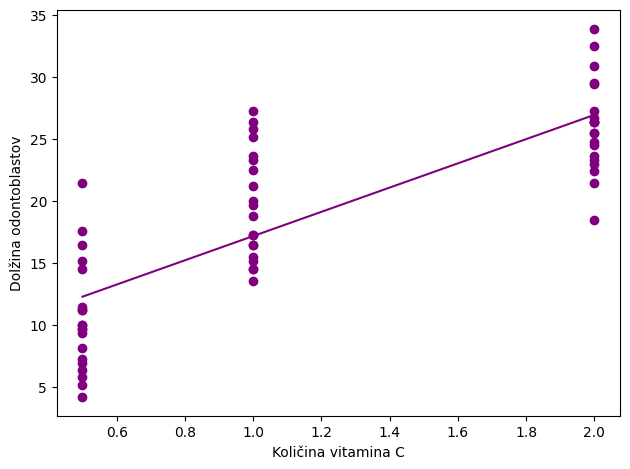
\includegraphics[scale=0.75]{Images/3a.png}
    \caption{Regresijski model iz točke (a)}
\end{figure}

\subsection*{(b)}
\addcontentsline{toc}{subsection}{\protect\numberline{}(b)}

Sedaj definiramo indikatorsko spremenljivko $\mathrm{način}$, ki je $0$, če je morski prašiček 
dobil vitamin C v obliki VC, sicer pa je $1$. Postavimo model 
$$\mathrm{dolžina} = \beta_0 + \beta_1 \cdot \mathrm{količina} + \beta_2 \cdot \mathrm{način}+ \beta_3 \cdot \mathrm{količina} \cdot \mathrm{način} + \varepsilon.$$
Od tod sledi, da je za morske prašičke, ki so dobili vitamin C v obliki VC, model enak
$$\mathrm{dolžina} = \beta_0 + \beta_1 \cdot \mathrm{količina},$$
za preostale pa 
$$\mathrm{dolžina} = (\beta_0 + \beta_2) + (\beta_1 + \beta_3) \cdot \mathrm{količina}.$$
Razlika v učinkovitosti VC in OJ je torej ravno koeficient $\beta_3$.


Sedaj pa nadaljujemo popolnoma enako kot pri prejšnji točki:
testiramo ničelno hipotezo 
$$H_0:\ \beta_3 = 0$$
proti alternativni hipotezi 
$$H_1:\ \beta_3 \neq 0.$$
Pa si poglejmo rezultat.

\begin{python}
    neodvisna_alt = zobje[["NACIN", "KOLICINA", "NACIN*KOLICINA"]]
    odvisna_alt = zobje["DOLZINA"]
    neodvisna_alt = sm.add_constant(neodvisna_alt)
    reg_alt = sm.OLS(odvisna_alt, neodvisna_alt).fit()
    koef_alt = reg_alt.params
    print(reg_alt.summary())
    c0_alt, c1_alt, c2_alt, c3_alt = koef_alt["const"], koef_alt["NACIN"], koef_alt["KOLICINA"], koef_alt["NACIN*KOLICINA"]

    y_vc = zobje_vc["DOLZINA"]
    x_vc = zobje_vc["KOLICINA"]
    y_oj = zobje_oj["DOLZINA"]
    x_oj = zobje_oj["KOLICINA"]

    x = np.linspace(0.5, 2.0, 100)
    fig, ax = plt.subplots()
    ax.set_facecolor('white')
    plt.scatter(x_vc, y_vc, c="red")
    plt.scatter(x_oj, y_oj, c="blue")
    rdeca = mpatches.Patch(color="red", label="VC")
    modra = mpatches.Patch(color="blue", label="OJ")
    plt.plot(x, c0_alt * np.ones(100) + c2_alt * x, "r")
    plt.plot(x, (c0_alt + c1_alt) * np.ones(100) + (c2_alt + c3_alt) * x, "b")
    ax.set_xlabel("Kolicina vitamina C")
    ax.set_ylabel("Dolzina odontoblastov")
    ax.legend(handles=[rdeca, modra])
    ax.grid(False)
    plt.tight_layout()
    plt.show()
\end{python}

\begin{figure}[H]
    \begin{center}
        \begin{tabular}{lSSSSSS} \toprule
            & $\mathrm{coef}$ & $\mathrm{std\ err}$ & {$t$} & {$P > |t|$} & {$0.025$} & {$0.975$} \\ \midrule
            const            &  3.2950   &   1.581   &   2.084   &   0.042    &   0.127   &    6.463\\
            NACIN            &  8.2550   &   2.236   &   3.691   &   0.001    &   3.775   &   12.735\\
            KOLICINA         & 11.7157   &   1.195   &   9.800   &   0.000    &   9.321   &   14.110\\
            NACIN*KOLICINA   & -3.9043   &   1.691   &  -2.309   &   0.025    &  -7.291   &   -0.518\\
            \bottomrule
        \end{tabular}   
    \end{center}
    \caption{Tabela koeficientov v regresijskem modelu iz točke (b)} 
\end{figure}

Iz tabele preberemo, da je $p$-vrednost koeficienta pri NAČIN*KOLICINA enaka $0.025$.
Če je $\alpha = 0.05$, potem ničelno hipotezo zavrnemo in zaključimo, da je način doziranja VC 
učinkovitejši od OJ. Če pa je $\alpha = 0.01$, potem ničelne hipoteze ne ovržemo in zaključimo, da ni dovolj dokazov,
da je kateri izmed načinov učinkovitejši. Razlika v naklonih torej ni statistično značilna.

\begin{figure}[H]
    \centering
    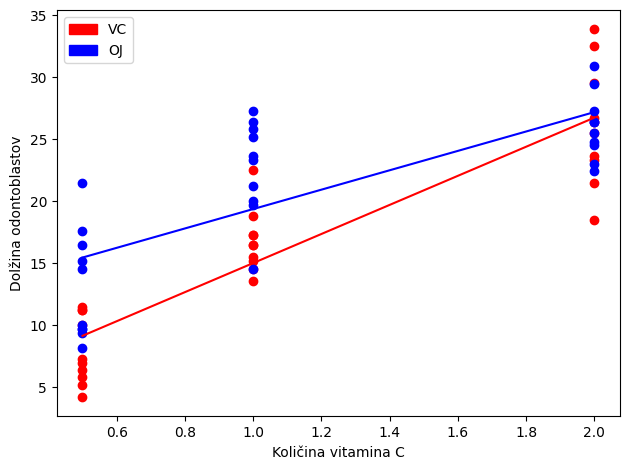
\includegraphics[scale=0.75]{Images/3b.png}
    {\caption{Regresijski model iz točke (b)}}
\end{figure}

\bibliographystyle{plain}
\bibliography{refs.bib}


\end{document}